
%----------------------------------------------------------------------------------------
%	PACKAGES AND OTHER DOCUMENT CONFIGURATIONS
%----------------------------------------------------------------------------------------

\documentclass[12pt]{article}
\usepackage[english]{babel}
\usepackage[utf8x]{inputenc}
\usepackage{amsmath}
\usepackage{graphicx}
\usepackage[colorinlistoftodos]{todonotes}
\usepackage{url}
\usepackage{listings}
\usepackage{minted}
\addto\captionsbrazilian{}

\begin{document}

\begin{titlepage}

\newcommand{\HRule}{\rule{\linewidth}{0.5mm}} % Defines a new command for the horizontal lines, change thickness here

\center % Center everything on the page
 
%----------------------------------------------------------------------------------------
%	HEADING SECTIONS
%----------------------------------------------------------------------------------------

\textsc{\normalsize Universidade Federal do Rio Grande do Sul}\\[1.0cm] % Name of your university/college
\textsc{\Large Verites}\\[0.2cm] % Major heading such as course name
\textsc{\large Verification, Validation and Test Group}\\[0.2cm] % Minor heading such as course title

%----------------------------------------------------------------------------------------
%	TITLE SECTION
%----------------------------------------------------------------------------------------

\HRule \\[0.4cm]
{ \huge \bfseries \LARGE{VERIGRAPH} \\ [1.0cm]
\emph{\large{Software specification and verification tool based on graph rewriting}}
}\\[0.5cm]

Version 1.0-rc01 \\[0.4cm] % Title of your document
\HRule \\[1.0cm]
 
%----------------------------------------------------------------------------------------
%	AUTHOR SECTION
%----------------------------------------------------------------------------------------

%\begin{minipage}{0.4\textwidth}
%\begin{flushleft} \large
%\emph{Alunos:}\\
%André Luiz Silveira Lucas %\textsc{Smith} % Your name
%Rafael 
%\end{flushleft}
%\end{minipage}
%~

%\begin{minipage}{0.4\textwidth}
%\begin{flushright} \large
%\emph{Supervisor:} \\
%Dr. James \textsc{Smith} % Supervisor's Name
%\end{flushright}
%\end{minipage}\\[2cm]

% If you don't want a supervisor, uncomment the two lines below and remove the section above
%\flushleft \Large \emph{Alunos:}\\ 
%João Marcos\\ 
%Maria Mara \\ % Your name

\center {\today}\\[2cm]


\includegraphics[scale = 3]{logo.jpg}\\[0.5cm]

\includegraphics[scale = 0.7]{LogoVerites.jpg}

 
%---------------------------------------------------------------------------------------- FOLHA DE ROSTO

\begin{titlepage}
\vfill
\begin{flushleft} 
{\large Andrei Costa \\
Guilherme Grochau Azzi \\
Jonas Santos Bezerra \\
Leila Ribeiro \\
Leonardo M. Rodrigues \\
Rodrigo Machado } \\ [5cm] 
{\Huge Verigraph Tutorial}
\vfill
\today
\end{flushleft}
\end{titlepage}

%-------------------------------------------------------------------
\vfill % Fill the rest of the page with whitespace

\end{titlepage}

\section{Installation}

\subsection{Requirements}
\begin{itemize}
\item GHC (The Glasgow Haskell Compiler) version 8.0.1 or superior
\item AGG (The Attributed Graph Grammar System) version 2.1: Download at \url{http://www.user.tu-berlin.de/o.runge/agg/}
\item Cabal 1.24 or Stack 1.1.2
\item Git Version Control System 
\end{itemize}

\subsection{On Linux}

Download the source code and checkout the latest stable version:
\begin{minted}{bash}
  $ git clone https://github.com/Verites/verigraph.git
  $ cd verigraph
  $ git checkout 1.0-rc01
\end{minted}


If you are using Cabal:
\begin{minted}{bash}
  $ cabal install
  $ export PATH=${PATH}:~/.cabal/bin
\end{minted}

If you are using Stack:
\begin{minted}{bash}
  $ stack install
  $ export PATH=${PATH}:~/.local/bin
\end{minted}

Add the PATH exportation also in your \texttt{.bashrc}

\subsection{On Windows}

\subsection{On MacOS}

\section{Graph Transformation Model}

\section{Global Configuration}

By default, \texttt{verigraph} will compute \textit{matches} and \textit{Epi-Pairs} with injective morphisms only, to compute with all kinds of morphisms use the \texttt{--all-matches} flag.

\section{Critical Pair Analysis}

\begin{minted}{bash}
  $ verigraph analysis
\end{minted}

\section{Concurrent Rules}

Using \texttt{AGG}, open the file \texttt{grammars/Server/server.ggx}, than right-click on the Grammar $>$ New $>$ Rule Sequence. \\

\noindent
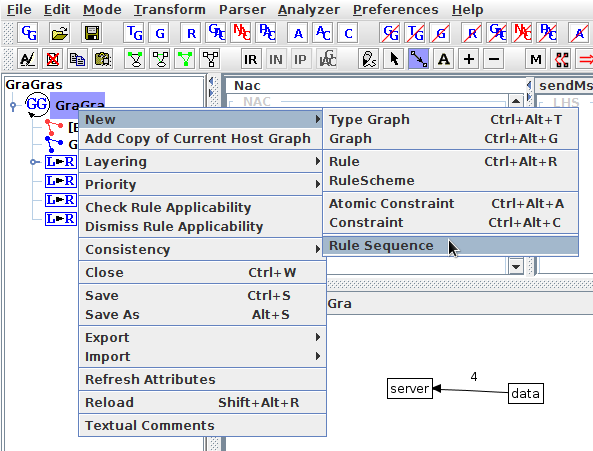
\includegraphics[scale = 0.6]{rule-sequence_01.png}

Right-click on the rule sequence created below the rules of the grammar, than click on \texttt{Show/Edit}, a new pop-up must open.\\

\noindent
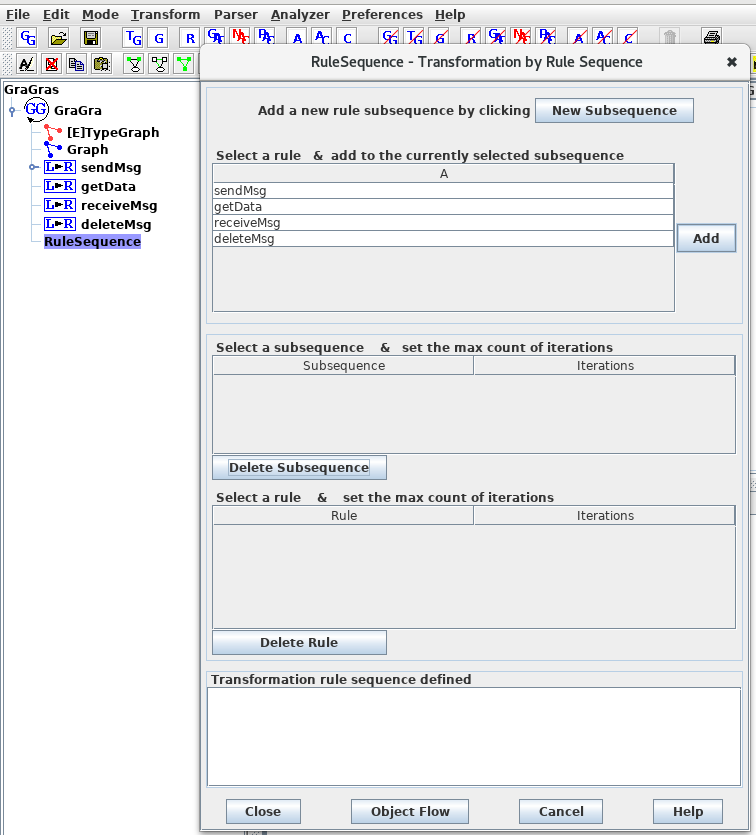
\includegraphics[scale = 0.5]{rule-sequence_02.png}\\

Click on \texttt{New Subsequence} button, a new row will be created at the \texttt{Select a subsequence} table. Select the subsequence to add the rules to it.

Once the subsequence was selected, we can add any rules in the \texttt{Select a rule} table. Select any rule(s) than click on the \texttt{Add} button, it is possible to add a rule more than once by either clicking on the \texttt{Add} button more than once or altering the number of \texttt{Iterations} for a particular rule in the \texttt{Select a rule} table. Once the rule sequence is defined, click on close and save the file.\\

\noindent
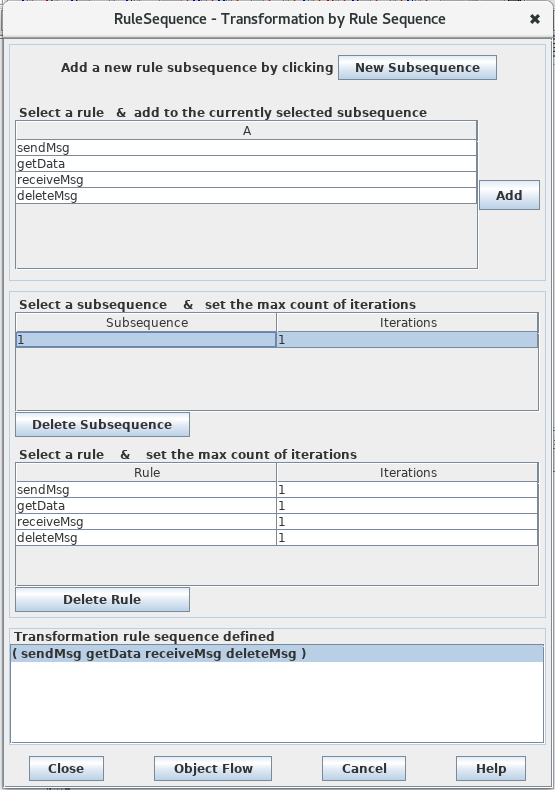
\includegraphics[scale = 0.6]{rule-sequence_03.png}\\

Now, we can use \texttt{verigraph} to compute the concurrent rule(s) for this rule sequence, the basic structure of the command is:

\begin{minted}{bash}
  $ verigraph concurrent-rule -o <outputFile>.ggx <inputFile>.ggx
\end{minted}

\subsection{Least disjoint}

To generate the concurrent rule with the least disjoint epi-pairs between each rule in the sequence run:

\begin{minted}{bash}
  $ verigraph concurrent-rule --max-rule -o output.ggx 
    grammars/Server/server.ggx
\end{minted}

Than open the \texttt{output.ggx} file in \texttt{AGG}, it must have one new rule that looks like this:\\

\noindent
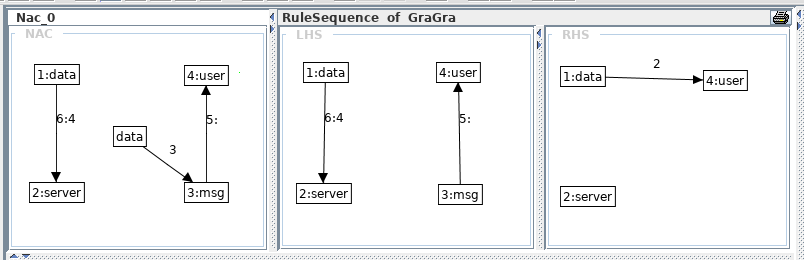
\includegraphics[scale = 0.6]{rule-sequence_04a.png}\\
\noindent
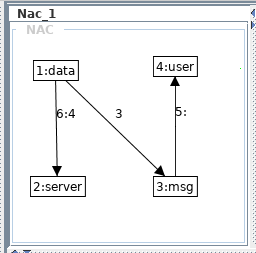
\includegraphics[scale = 0.6]{rule-sequence_04b.png}\\

\subsection{Dependent rules}

To generate the concurrent rules where there are dependencies between the rules in the sequence run:

\begin{minted}{bash}
  $ verigraph concurrent-rule --all-rules --by-dependency -o output.ggx 
    grammars/Server/server.ggx
\end{minted}

The output file must have two new rules, one identical (isomorphic) to the one in the previous example, and one other that looks like this:\\

\noindent
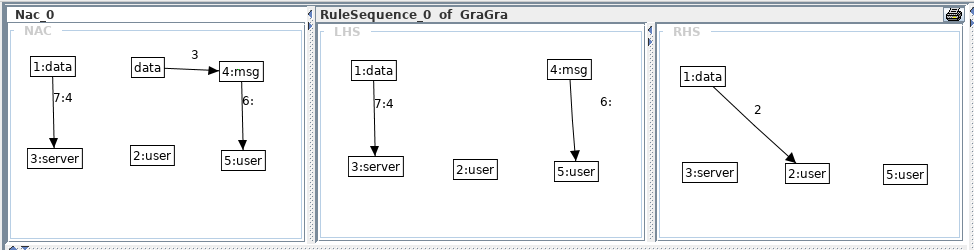
\includegraphics[scale = 0.5]{rule-sequence_05a.png}\\
\noindent
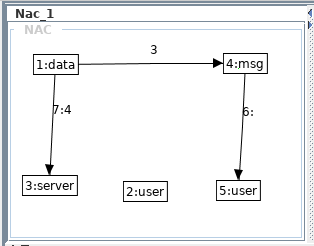
\includegraphics[scale = 0.5]{rule-sequence_05b.png}\\

\subsection{Other rules}

To generate all the concurrent rules for this example, run:

\begin{minted}{bash}
  $ verigraph concurrent-rule -o output.ggx grammars/Server/server.ggx
\end{minted}

Note this operation may take a while, since it will calculate all possible overlaps between the rules in the sequence (in this particular case 1202 rules)\footnote{We are currently working in graph constraints and multiplicity to improve the generation of concurrent rules}.

All the previous examples were constructed using only injective morphisms, to calculate with all kinds of morphisms use the flag \texttt{--all-matches} after the \texttt{verigraph} command.

\section{Second Order}

\begin{minted}{bash}
  $ verigraph snd-order
\end{minted}

%\section{Model Checking}

%\begin{minted}{bash}
%  $ verigraph-mcheck
%\end{minted}
\end{document}